\documentclass{article}

\usepackage{natbib}
\usepackage{fullpage}
\usepackage{hyperref}
\usepackage{amsmath}
\usepackage{dsfont}
\newcommand{\1}{\mathds{1}}
\newcommand{\E}{\mathrm{E}}
\usepackage{booktabs}
\usepackage[flushleft]{threeparttable}
\newcommand{\mynote}{\item \leavevmode\kern-\scriptspace\kern-\labelsep}
\usepackage{graphicx}
\newcommand{\myrotate}[1]{#1}
\newcommand{\PreserveBackslash}[1]{\let\temp=\\#1\let\\=\temp}
\newcommand{\mycell}[1]{\parbox[m]{1.1in}{\PreserveBackslash\raggedright \vspace{7pt} #1 \vspace{7pt}}}
\usepackage{multirow}
\usepackage{stfloats}

\title{
  Stack Overflow Badges and User Behavior
}
\author{
  Andrew Marder
}
\date{\today}

\begin{document}

\maketitle

\begin{abstract}
Does gamification work? This paper examines how Stack Overflow users behave when earning badges. A regression analysis of user activity logs shows users change their contribution amounts when earning some badges but not others. This paper adds new support to the growing literature that gamification works, but its efficacy is context-dependent \citep{Hamari}. Alternative methods for motivating user contributions are considered.
\end{abstract}

\section{Introduction}

Stack Overflow is a question and answer community designed for programmers. It is the largest of 130 communities in the Stack Exchange network. Created in 2008, the knowledge organized by Stack Overflow has become a valuable resource for software developers. On January 20, 2015, \citet{Spoelsky2015} announced that Stack Exchange had raised \$40 million in venture capital funding. Stack Overflow gives users who ask questions access to expert technical help, while users who answer questions build their reputation for technical expertise.

\citet{Deterding2011} define ``\textit{gamification} as the use of game design elements in non-game contexts.'' Stack Overflow gamifies the process of asking and answering questions as follows. A user earns reputation points when another user votes on her posts (5 points when a question is voted up, 10 points when an answer is voted up, 15 points when an answer is accepted, and 2 points when an edit is approved). As a user earns reputation points she unlocks privileges on the site. For instance, a user must have at least 15 reputation points to vote up a question or answer.\footnote{A full list of privileges and the necessary reputation points is available at \url{http://stackoverflow.com/help/privileges}.} Users are awarded badges for special achievements. For example, one receives the \textit{Informed} badge by reading the tour page.\footnote{The Stack Overflow tour can be found at \url{http://stackoverflow.com/tour}, and all badges are listed on \url{http://stackoverflow.com/help/badges}.}

This paper takes a first step along the path of applying econometric analysis to publicly available Stack Overflow data \cite{se-dump}. Do badges motivate users to contribute to the site? Which badges are most effective? What types of user contributions are responsive to gamification? To begin answering these questions, I study how users behave around the time they are awarded badges.

\section{Motivating Contributions}

\citet{Kraft-Todd} survey the literature on field experiments designed
to promote cooperation in social dilemmas. Examples of social dilemmas include voter turnout,
environmental protection, and universal healthcare. Table
\ref{tab:kraft-todd} describes the four categories they use to
classify interventions.

\begin{table}[h!tbp]
  \centering
  \renewcommand{\arraystretch}{2}
  \caption{Four types of intervention used to promote contributions to a public good.}
  \label{tab:kraft-todd}
  \begin{tabular}{r|c|c|}

    \multicolumn{1}{c}{} & \multicolumn{1}{c}{\textit{Material-benefit}} & \multicolumn{1}{c}{\textit{Social-benefit}} \\
    \cline{2-3}

    \myrotate{\textit{Self-focused}} & \mycell{ Material rewards \\ \\ Cash or gifts provided in exchange for contributing } & \mycell{Observability \\ \\ Others informed about your contribution decisions} \\

    \cline{2-3}

    \myrotate{\textit{Other-focused}} & \mycell{ Increased efficacy \\ \\ Matching/seed funds provided, or benefit to others emphasized } & \mycell{Descriptive norms \\ \\ You are informed about the contribution decisions of others} \\

    \cline{2-3}
  \end{tabular}
\end{table}

\begin{table}
  \begin{threeparttable}
    % \ra{1.2}
    \caption{Badges of interest}
    \label{tab:badges}
    \begin{tabular}{@{}llccc@{}}
      \toprule
      Name & Description & Awarded & Introduced & Dropped \\
      \midrule
      Strunk \& White & Edited 80 posts & 7,073 & 2008-09-15 & 0.00 \\
      Copy Editor & Edited 500 posts & 1,288 & 2010-07-09 & 0.04 \\
      Archaeologist & Edited 100 posts that were inactive for 6 months & 691 & 2011-08-15 & 0.05 \\
      Curious & Asked a well-received question on 5 separate days & 138,264 & 2014-07-02 & 0.86 \\
      Inquisitive & Asked a well-received question on 30 separate days & 14,081 & 2014-07-02 & 0.92 \\
      Socratic & Asked a well-received question on 100 separate days & 1,240 & 2014-07-02 & 0.93 \\
      \bottomrule
    \end{tabular}
    \begin{tablenotes}
    \item The six badges considered in this paper were introduced to the Stack Overflow site at different times. The Strunk \& White badge was first awarded on September 15, 2008, while the three badges for asking questions were all introduced on July 2, 2014. Since the badges for asking questions were added to the site so recently many users who have been awarded these badges earned them for actions taken before the badge was introduced. For instance, 86\% of users who earned the Curious badge were awarded the badge for actions taken before July 2, 2014. I drop these users from the analysis as they have no incentive to change their behavior to earn the Curious badge.
    \end{tablenotes}
  \end{threeparttable}
\end{table}


Focusing on the experiments surveyed by \citet{Kraft-Todd}, interventions that provided material benefits led to mixed results while interventions that provided social benefits were consistently effective at promoting cooperation. The general categories of Table \ref{tab:kraft-todd} hint at some of the specific reasons why users might contribute to Stack Overflow:
\begin{enumerate}
\item Material rewards: A user might contribute to Stack Overflow to
  signal her technical ability to potential employers. By
  contributing to Stack Overflow she increases the probability of
  finding better employment opportunities, leading to material
  rewards.
\item Increased efficacy: By emphasizing how high quality
  answers help others solve similar problems, Stack
  Overflow can motivate other-interested individuals to contribute. \cite{Gerbasi}
\item Observability: Contributions to the platform are publicized
  through the reputation and badge system. If a user is concerned
  about how others perceive her on the site (generous, competent, \dots),
  she may be motivated to contribute.
\item Descriptive norms: If a user is concerned about how her
  contributions compare to the contributions of others, the reputation
  leaderboards may motivate her to contribute.\footnotetext{A question is \textit{well-received} if it is open and has a score greater than 0. \url{http://meta.stackexchange.com/questions/234259/asking-days-badges}}\footnote{The Stack Exchange leaderboards are online at \url{http://stackexchange.com/leagues}.}
\end{enumerate}
This is not an exhaustive list of why users contribute to Stack Overflow. However, it will be useful when considering why users increase contributions when receiving some but not all badges.

\section{Methods}

\citet{Grant2013} present empirical evidence that three badges awarded for editing encourage recipients to make more edits in the two months preceding receipt of the badge compared to the two months after receiving the badge. This paper extends their findings by examining all types of user activity (posting questions, posting answers, and editing posts), and exploring the impact of three new badges awarded for asking questions. Table \ref{tab:badges} describes the six badges considered in this paper.

Let $y_{it}$ be the number of edits user $i$ makes on day $t$, and $t_i^*$ denote the day user $i$ receives the badge of interest. Following the approach of \citet{Jacobson1993}, I regress the number of edits user $i$ makes on day $t$ on a user fixed effect $\alpha_i$, a set of dummy variables indicating whether the user received the badge on day $t-k$, and day of the week effects $\gamma_j$
\begin{equation}
\log(1 + y_{it}) = \; \alpha_i + \sum_{k=-29}^{30} \1 \{ t = t_i^* + k \} \delta_k \; + \sum_{j=1}^6 \1 \{ t \bmod 7 = j \} \gamma_j + \epsilon_{it}.
\end{equation}
The model parameters are estimated using an ordinary least squares regression, and standard errors are clustered at the user level.

Define $f(k)$ to be the expected number of actions taken on the $k$'th day since receiving the badge
\begin{equation}
f(k) = \E \left[ \log(1 + y_{it}) \; | \; t=t^*_i + k \right].
\end{equation}
The predicted number of actions $\hat{f(k)}$ is presented in Figure \ref{fig:badges}. The 95\% confidence interval is depicted as a gray band around the linear prediction, standard errors were calculated using the delta method \citep{Williams2012}.

\section{Results}

\begin{figure*}
  \centering
  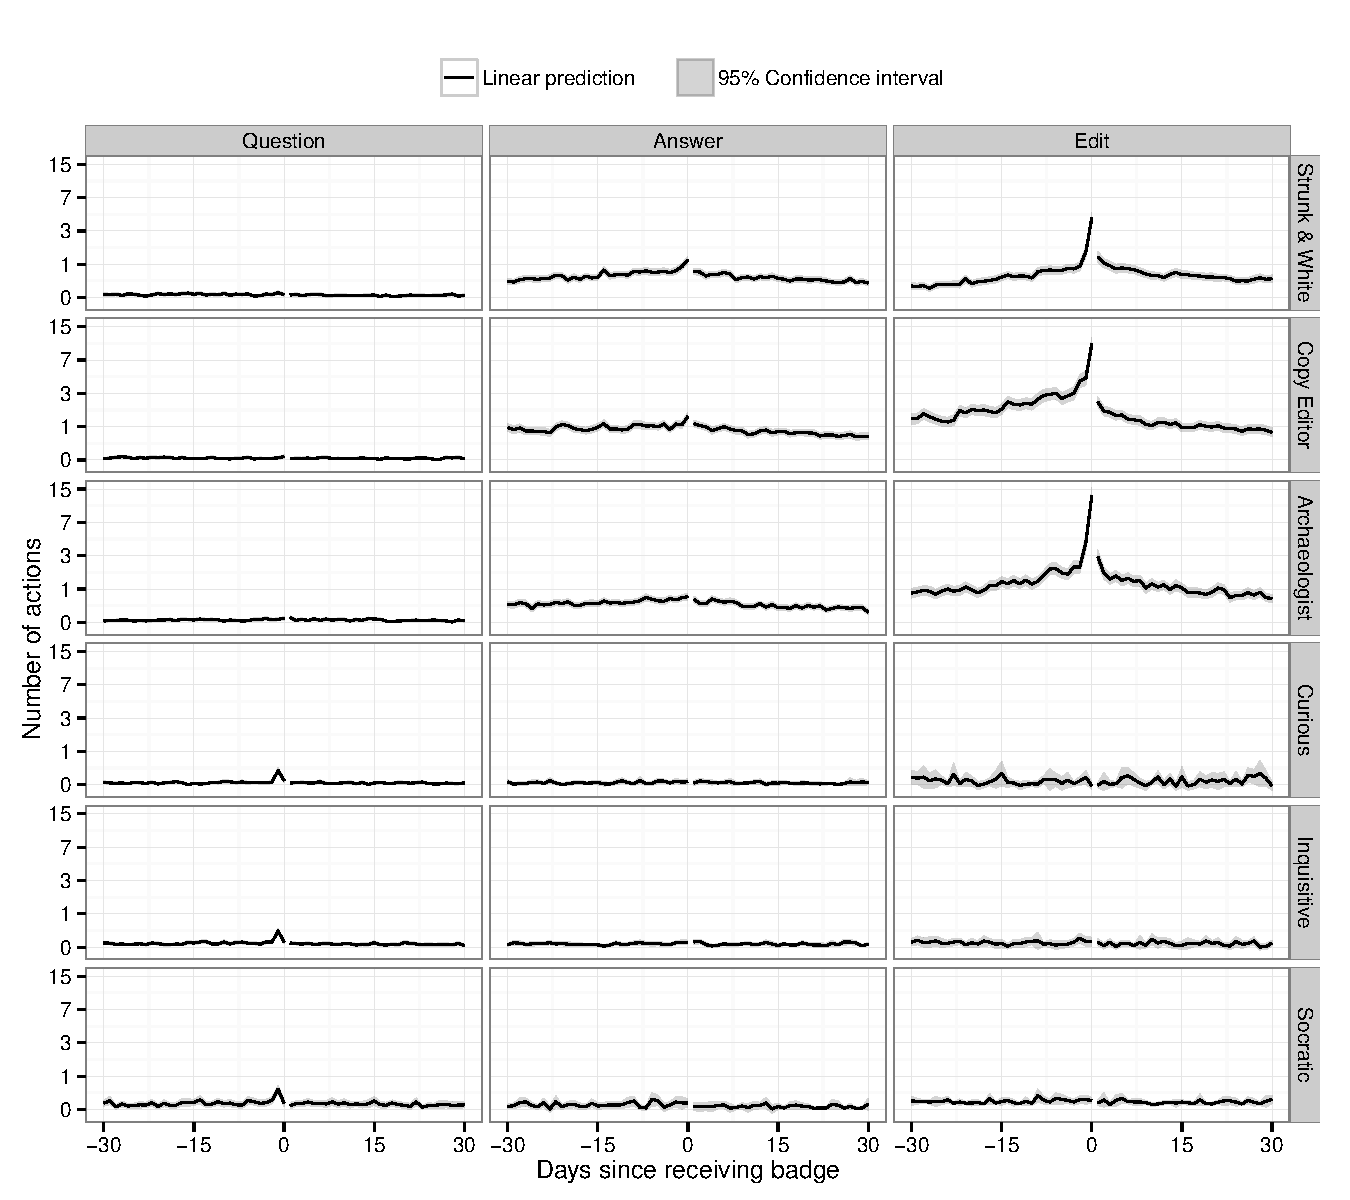
\includegraphics[width=\textwidth]{../figures/badges.pdf}
  \caption{User activity over time \label{fig:badges}}
\end{figure*}

The first three rows of Figure \ref{fig:badges} illustrate how user activity changes around the time one earns a badge for editing. Each row is labeled with the name of the focal badge (\textit{Strunk \& White}, \textit{Copy Editor}, and \textit{Archaeologist}). There is one column for each type of user action (posting a question, posting an answer, or editing a post). The figure confirms the findings of \citet{Grant2013}. Editing increases gradually before receiving a badge for editing, with a large jump in activity on the award day. We also see that editing drops quickly after receiving the badge and gradually declines over time. It is interesting to see how few questions were asked by the recipients of the editing badges, and that the rate of answering questions has a very slight increase leading up to receiving the badge and a similarly slight decrease after receiving the badge.

The results for the question-focused badges, \textit{Curious}, \textit{Inquisitive}, and \textit{Socratic}, are quite different. In general, recipients of these badges are not particularly active on the site. The average level of questions, answers, and edits made all hover near zero. The uptick in questions asked on the day before receiving the badge is mechanical. Many users who earn these badges ask a question the day before they earn the badge.

\section{Conclusion}

When interpreting the empirical results of this paper, please recall Holland and Rubin's motto "no causation without manipulation" \citep{Holland1986}. There is no manipulation of the explanatory variable in this study, consequently we have not identified the causal effect of badges. To estimate the causal impact of badges on user activity we need to find a source of exogenous variation \citep{Miller2013}.

This paper confirms the empirical observation of \citet{Grant2013}. On average, users who receive a badge for editing make more edits in the 30 days prior to receiving the badge compared to the 30 days after receiving the badge. In addition, we find that recipients of the editing badges ask almost no questions, and answer about one question each day. Finally, we show that users who receive badges for asking questions behave differently. In particular, we found that users do not appear motivated to change their activity levels to earn badges for asking questions.

Although Stack Overflow has design elements that exemplify each of the four motivators outlined by \citet{Grant2013}, badges awarded for asking questions appear unable to increase the number of questions posted to the site. Asking a good question is difficult, it requires ``search and research'' \cite{so-ask}. One feature that might increase the number of questions posted is adding support for anonymous questions. Allowing a user to remove the observability of her action would help her avoid the social cost of posting a poorly researched question. A careful system of anonymous questions would have to balance the benefit of increasing the number of questions asked, with the cost of lower quality questions on average.

\section*{Acknowledgements}

The author would like to thank three anonymous reviewers for helpful comments and suggestions, and Harvard Business School for financial support.

\bibliographystyle{plainnat}
\bibliography{clean}

\end{document}
